\documentclass[a4paper]{article}

%================================================================================================================================
%
% Packages
%
%================================================================================================================================

\usepackage[T1]{fontenc} 	% pour caractères accentués
\usepackage[utf8]{inputenc}  % encodage utf8
\usepackage[french]{babel}	% langue : français
\usepackage{fourier}			% caractères plus lisibles
\usepackage[dvipsnames]{xcolor} % couleurs
\usepackage{fancyhdr}		% réglage header footer
\usepackage{needspace}		% empêcher sauts de page mal placés
\usepackage{graphicx}		% pour inclure des graphiques
\usepackage{enumitem,cprotect}		% personnalise les listes d'items (nécessaire pour ol, al ...)
\usepackage{hyperref}		% Liens hypertexte
\usepackage{pstricks,pst-all,pst-node,pstricks-add,pst-math,pst-plot,pst-tree,pst-eucl} % pstricks
\usepackage[a4paper,includeheadfoot,top=2cm,left=3cm, bottom=2cm,right=3cm]{geometry} % marges etc.
\usepackage{comment}			% commentaires multilignes
\usepackage{amsmath,environ} % maths (matrices, etc.)
\usepackage{amssymb,makeidx}
\usepackage{bm}				% bold maths
\usepackage{tabularx}		% tableaux
\usepackage{colortbl}		% tableaux en couleur
\usepackage{fontawesome}		% Fontawesome
\usepackage{environ}			% environment with command
\usepackage{fp}				% calculs pour ps-tricks
\usepackage{multido}			% pour ps tricks
\usepackage[np]{numprint}	% formattage nombre
\usepackage{tikz,tkz-tab} 			% package principal TikZ
\usepackage{pgfplots}   % axes
\usepackage{mathrsfs}    % cursives
\usepackage{calc}			% calcul taille boites
\usepackage[scaled=0.875]{helvet} % font sans serif
\usepackage{svg} % svg
\usepackage{scrextend} % local margin
\usepackage{scratch} %scratch
\usepackage{multicol} % colonnes
%\usepackage{infix-RPN,pst-func} % formule en notation polanaise inversée
\usepackage{listings}

%================================================================================================================================
%
% Réglages de base
%
%================================================================================================================================

\lstset{
language=Python,   % R code
literate=
{á}{{\'a}}1
{à}{{\`a}}1
{ã}{{\~a}}1
{é}{{\'e}}1
{è}{{\`e}}1
{ê}{{\^e}}1
{í}{{\'i}}1
{ó}{{\'o}}1
{õ}{{\~o}}1
{ú}{{\'u}}1
{ü}{{\"u}}1
{ç}{{\c{c}}}1
{~}{{ }}1
}


\definecolor{codegreen}{rgb}{0,0.6,0}
\definecolor{codegray}{rgb}{0.5,0.5,0.5}
\definecolor{codepurple}{rgb}{0.58,0,0.82}
\definecolor{backcolour}{rgb}{0.95,0.95,0.92}

\lstdefinestyle{mystyle}{
    backgroundcolor=\color{backcolour},   
    commentstyle=\color{codegreen},
    keywordstyle=\color{magenta},
    numberstyle=\tiny\color{codegray},
    stringstyle=\color{codepurple},
    basicstyle=\ttfamily\footnotesize,
    breakatwhitespace=false,         
    breaklines=true,                 
    captionpos=b,                    
    keepspaces=true,                 
    numbers=left,                    
xleftmargin=2em,
framexleftmargin=2em,            
    showspaces=false,                
    showstringspaces=false,
    showtabs=false,                  
    tabsize=2,
    upquote=true
}

\lstset{style=mystyle}


\lstset{style=mystyle}
\newcommand{\imgdir}{C:/laragon/www/newmc/assets/imgsvg/}
\newcommand{\imgsvgdir}{C:/laragon/www/newmc/assets/imgsvg/}

\definecolor{mcgris}{RGB}{220, 220, 220}% ancien~; pour compatibilité
\definecolor{mcbleu}{RGB}{52, 152, 219}
\definecolor{mcvert}{RGB}{125, 194, 70}
\definecolor{mcmauve}{RGB}{154, 0, 215}
\definecolor{mcorange}{RGB}{255, 96, 0}
\definecolor{mcturquoise}{RGB}{0, 153, 153}
\definecolor{mcrouge}{RGB}{255, 0, 0}
\definecolor{mclightvert}{RGB}{205, 234, 190}

\definecolor{gris}{RGB}{220, 220, 220}
\definecolor{bleu}{RGB}{52, 152, 219}
\definecolor{vert}{RGB}{125, 194, 70}
\definecolor{mauve}{RGB}{154, 0, 215}
\definecolor{orange}{RGB}{255, 96, 0}
\definecolor{turquoise}{RGB}{0, 153, 153}
\definecolor{rouge}{RGB}{255, 0, 0}
\definecolor{lightvert}{RGB}{205, 234, 190}
\setitemize[0]{label=\color{lightvert}  $\bullet$}

\pagestyle{fancy}
\renewcommand{\headrulewidth}{0.2pt}
\fancyhead[L]{maths-cours.fr}
\fancyhead[R]{\thepage}
\renewcommand{\footrulewidth}{0.2pt}
\fancyfoot[C]{}

\newcolumntype{C}{>{\centering\arraybackslash}X}
\newcolumntype{s}{>{\hsize=.35\hsize\arraybackslash}X}

\setlength{\parindent}{0pt}		 
\setlength{\parskip}{3mm}
\setlength{\headheight}{1cm}

\def\ebook{ebook}
\def\book{book}
\def\web{web}
\def\type{web}

\newcommand{\vect}[1]{\overrightarrow{\,\mathstrut#1\,}}

\def\Oij{$\left(\text{O}~;~\vect{\imath},~\vect{\jmath}\right)$}
\def\Oijk{$\left(\text{O}~;~\vect{\imath},~\vect{\jmath},~\vect{k}\right)$}
\def\Ouv{$\left(\text{O}~;~\vect{u},~\vect{v}\right)$}

\hypersetup{breaklinks=true, colorlinks = true, linkcolor = OliveGreen, urlcolor = OliveGreen, citecolor = OliveGreen, pdfauthor={Didier BONNEL - https://www.maths-cours.fr} } % supprime les bordures autour des liens

\renewcommand{\arg}[0]{\text{arg}}

\everymath{\displaystyle}

%================================================================================================================================
%
% Macros - Commandes
%
%================================================================================================================================

\newcommand\meta[2]{    			% Utilisé pour créer le post HTML.
	\def\titre{titre}
	\def\url{url}
	\def\arg{#1}
	\ifx\titre\arg
		\newcommand\maintitle{#2}
		\fancyhead[L]{#2}
		{\Large\sffamily \MakeUppercase{#2}}
		\vspace{1mm}\textcolor{mcvert}{\hrule}
	\fi 
	\ifx\url\arg
		\fancyfoot[L]{\href{https://www.maths-cours.fr#2}{\black \footnotesize{https://www.maths-cours.fr#2}}}
	\fi 
}


\newcommand\TitreC[1]{    		% Titre centré
     \needspace{3\baselineskip}
     \begin{center}\textbf{#1}\end{center}
}

\newcommand\newpar{    		% paragraphe
     \par
}

\newcommand\nosp {    		% commande vide (pas d'espace)
}
\newcommand{\id}[1]{} %ignore

\newcommand\boite[2]{				% Boite simple sans titre
	\vspace{5mm}
	\setlength{\fboxrule}{0.2mm}
	\setlength{\fboxsep}{5mm}	
	\fcolorbox{#1}{#1!3}{\makebox[\linewidth-2\fboxrule-2\fboxsep]{
  		\begin{minipage}[t]{\linewidth-2\fboxrule-4\fboxsep}\setlength{\parskip}{3mm}
  			 #2
  		\end{minipage}
	}}
	\vspace{5mm}
}

\newcommand\CBox[4]{				% Boites
	\vspace{5mm}
	\setlength{\fboxrule}{0.2mm}
	\setlength{\fboxsep}{5mm}
	
	\fcolorbox{#1}{#1!3}{\makebox[\linewidth-2\fboxrule-2\fboxsep]{
		\begin{minipage}[t]{1cm}\setlength{\parskip}{3mm}
	  		\textcolor{#1}{\LARGE{#2}}    
 	 	\end{minipage}  
  		\begin{minipage}[t]{\linewidth-2\fboxrule-4\fboxsep}\setlength{\parskip}{3mm}
			\raisebox{1.2mm}{\normalsize\sffamily{\textcolor{#1}{#3}}}						
  			 #4
  		\end{minipage}
	}}
	\vspace{5mm}
}

\newcommand\cadre[3]{				% Boites convertible html
	\par
	\vspace{2mm}
	\setlength{\fboxrule}{0.1mm}
	\setlength{\fboxsep}{5mm}
	\fcolorbox{#1}{white}{\makebox[\linewidth-2\fboxrule-2\fboxsep]{
  		\begin{minipage}[t]{\linewidth-2\fboxrule-4\fboxsep}\setlength{\parskip}{3mm}
			\raisebox{-2.5mm}{\sffamily \small{\textcolor{#1}{\MakeUppercase{#2}}}}		
			\par		
  			 #3
 	 		\end{minipage}
	}}
		\vspace{2mm}
	\par
}

\newcommand\bloc[3]{				% Boites convertible html sans bordure
     \needspace{2\baselineskip}
     {\sffamily \small{\textcolor{#1}{\MakeUppercase{#2}}}}    
		\par		
  			 #3
		\par
}

\newcommand\CHelp[1]{
     \CBox{Plum}{\faInfoCircle}{À RETENIR}{#1}
}

\newcommand\CUp[1]{
     \CBox{NavyBlue}{\faThumbsOUp}{EN PRATIQUE}{#1}
}

\newcommand\CInfo[1]{
     \CBox{Sepia}{\faArrowCircleRight}{REMARQUE}{#1}
}

\newcommand\CRedac[1]{
     \CBox{PineGreen}{\faEdit}{BIEN R\'EDIGER}{#1}
}

\newcommand\CError[1]{
     \CBox{Red}{\faExclamationTriangle}{ATTENTION}{#1}
}

\newcommand\TitreExo[2]{
\needspace{4\baselineskip}
 {\sffamily\large EXERCICE #1\ (\emph{#2 points})}
\vspace{5mm}
}

\newcommand\img[2]{
          \includegraphics[width=#2\paperwidth]{\imgdir#1}
}

\newcommand\imgsvg[2]{
       \begin{center}   \includegraphics[width=#2\paperwidth]{\imgsvgdir#1} \end{center}
}


\newcommand\Lien[2]{
     \href{#1}{#2 \tiny \faExternalLink}
}
\newcommand\mcLien[2]{
     \href{https~://www.maths-cours.fr/#1}{#2 \tiny \faExternalLink}
}

\newcommand{\euro}{\eurologo{}}

%================================================================================================================================
%
% Macros - Environement
%
%================================================================================================================================

\newenvironment{tex}{ %
}
{%
}

\newenvironment{indente}{ %
	\setlength\parindent{10mm}
}

{
	\setlength\parindent{0mm}
}

\newenvironment{corrige}{%
     \needspace{3\baselineskip}
     \medskip
     \textbf{\textsc{Corrigé}}
     \medskip
}
{
}

\newenvironment{extern}{%
     \begin{center}
     }
     {
     \end{center}
}

\NewEnviron{code}{%
	\par
     \boite{gray}{\texttt{%
     \BODY
     }}
     \par
}

\newenvironment{vbloc}{% boite sans cadre empeche saut de page
     \begin{minipage}[t]{\linewidth}
     }
     {
     \end{minipage}
}
\NewEnviron{h2}{%
    \needspace{3\baselineskip}
    \vspace{0.6cm}
	\noindent \MakeUppercase{\sffamily \large \BODY}
	\vspace{1mm}\textcolor{mcgris}{\hrule}\vspace{0.4cm}
	\par
}{}

\NewEnviron{h3}{%
    \needspace{3\baselineskip}
	\vspace{5mm}
	\textsc{\BODY}
	\par
}

\NewEnviron{margeneg}{ %
\begin{addmargin}[-1cm]{0cm}
\BODY
\end{addmargin}
}

\NewEnviron{html}{%
}

\begin{document}
\meta{url}{/exercices/matrices-bac-blanc-es-l-sujet-4-maths-cours-2018-spe/}
\meta{pid}{10508}
\meta{titre}{Matrices - Bac blanc ES/L Sujet 4 - Maths-cours 2018 (spé)}
\meta{type}{exercices}
%
\begin{h2}Exercice 3 (5 points)\end{h2}
\par      
\textbf{Candidats ayant suivi l'enseignement de spécialité}
\par
%============================================================================================================================
%
\TitreC{Partie A}
%
%============================================================================================================================
\par
Un service de garde d'enfants dispose d'un toboggan dans son espace de jeux.
\par
Le profil de ce toboggan peut être représenté, dans un repère orthonormé d'unité 1 mètre, par la courbe $\mathscr{C}$ d'une fonction $f$ définie sur l'intervalle $[0~;~3]$ à l'aide d'une formule du type :
\[ f(x)=ax^3+bx^2+cx+d \]
où $a, b, c$ et $d$ sont quatre réels.
\par
\begin{center}
     \begin{extern}%width="550" alt="Courbe fonction toboggan"
          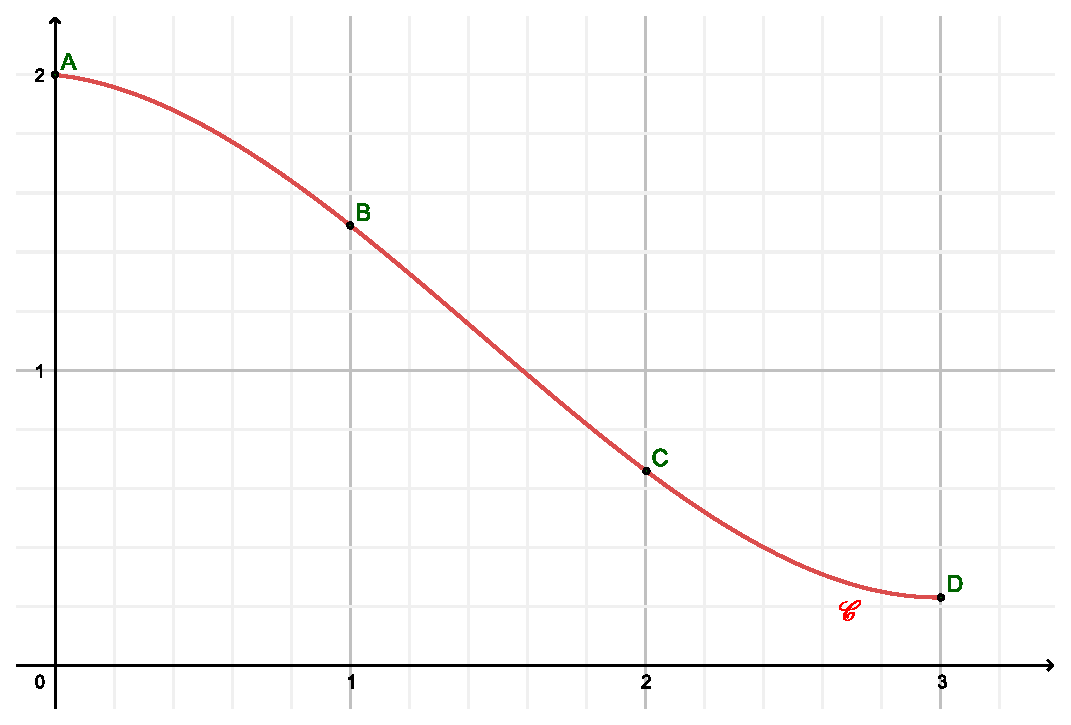
\includegraphics[width=0.9\textwidth]{images/BBESL-spe-4-1}% gbb 1 unite=5cm
     \end{extern}
\end{center}
\par
La courbe $\mathscr{C}$ passe par les points $A(0~;~2)$, $B(1~;~1,49)$, $C(2~;~0,66)$ et $D(3~;~0,23)$.
\par
\begin{enumerate}
     \item %1
     Montrer que les réels $a, b, c$ et $d$ sont les solutions d'un système (S) de quatre équations que l'on déterminera.
     \item %2
     On pose :
     \begin{center}
          $M = \begin{pmatrix}
               0 &0 &0 &1 \\
               1 &1 &1 &1 \\
               8 &4 &2 &1 \\
          27 &9 &3 &1  \end{pmatrix}$,
          $     X = \begin{pmatrix}
               a \\
               b \\
               c \\
          d  \end{pmatrix} $
          et
          $   Y = \begin{pmatrix}
               2 \\
               1,49 \\
               0,66 \\
          0,23 \end{pmatrix}$
     \end{center}
     Donner une écriture matricielle du système (S) utilisant les matrices $M, X$ et $Y$
     \item %3
     \`A l'aide d'une calculatrice, vérifier que la matrice $M$ est inversible et déterminer $M^{-1}$.
     \item %4
     Calculer $a, b, c$ et $d$ et en déduire l'expression de $f(x)$.
     \par
\end{enumerate}
\par
%============================================================================================================================
%
\TitreC{Partie B}
%
%============================================================================================================================
\par
Cette garderie propose des déjeuners pour les enfants le mercredi après-midi.
\par
Les enfants ont le choix entre deux menus : le menu \textit{steak haché - frites} et le menu \textit{plat du jour}.
\par
On a remarqué que :
\par
\begin{itemize}
     \item
     si un enfant a choisi le menu \textit{steak haché - frites} un mercredi, la probabilité qu'il choisisse à nouveau ce menu le mercredi suivant est de 0,5 ;
     \item
     si un enfant a choisi le menu \textit{plat du jour} un mercredi, la probabilité qu'il choisisse à nouveau ce menu le mercredi suivant est de 0,7.
\end{itemize}
\par
On sélectionne un enfant au hasard et on note $A$ l'état \og l'enfant choisit le menu \textit{steak haché - frites} \fg{} et $B$ l'état \og l'enfant choisit le menu \textit{plat du jour} \fg{}.
\par
\begin{enumerate}
     \item Traduire les données de l'énoncé par un graphe probabiliste de sommets $A$ et $B$.
     \item Écrire la matrice de transition $M$ de ce graphe en respectant l'ordre alphabétique des sommets.
     \item Montrer que ce graphe admet un état stable que l'on déterminera.\\
     Interpréter ce résultat.
\end{enumerate}
\begin{corrige}
     %============================================================================================================================
     %
     \TitreC{Partie A}
     %
     %============================================================================================================================
     \par
     \begin{enumerate}
          \item %1
          Comme la courbe $\mathscr{C}$ passe par les points $A(0~;~2)$, ${B(1~;~1,49)}$, ${C(2~;~0,66)}$ et ${D(3~;~0,23)}$, on a
          ${f(0)=2}$, ${f(1)=1,49}$, ${f(2)=0,66}$ et ${f(3)=0,23}$.
          \par
          Or :
          \par
          $f(0)=a \times 0^3 +b \times 0^2 + c \times 0 + d $\nosp$= d$ ;\\
          $f(1)=a \times 1^3 +b \times 1^2 + c \times 1 + d $\nosp$= a+b+c+d$ ;\\
          $f(2)=a \times 2^3 +b \times 2^2 + c \times 2 + d $\nosp$= 8a+4b+2c+d$ ;\\
          $f(3)=a \times 3^3 +b \times 3^2 + c \times 3 + d $\nosp$= 27a+9b+3c+d$.\\
          \par
          Donc $a, b, c$ et $d$  sont les solutions du système (S) :
          \par
          \[\left\{\begin{array}{c c c c c c c c c}
                    &&&&&&d& = &2\\
                    a&+&b&+&c&+&d& = &1,49\\
                    8a&+&4b&+&2c&+&d& = &0,66\\
                    27a&+&9b&+&3c&+&d& = &0,23
          \end{array}\right.\]
          \item %2
          Le produit de matrices $ M \times X $ est égal à :
          \par
          $ M \times X = \begin{pmatrix}
               0 &0 &0 &1 \\
               1 &1 &1 &1 \\
               8 &4 &2 &1 \\
          27 &9 &3 &1  \end{pmatrix} \times
          \begin{pmatrix}
               a \\
               b \\
               c \\
               d  \end{pmatrix}  = \begin{pmatrix}
               d \\
               a+b+c+d \\
               8a+4b+2c+d \\
          27a+9b+3c+d \end{pmatrix}
          $
          \par
          Le système $(S)$ peut donc s'écrire sous forme matricielle :
          \[ M \times X = Y. \]
          \item %3
          \`A la calculatrice, on constate que la matrice $M$ est inversible et que :
          \[ M^{-1}=  \begin{pmatrix}
               -1/6 &1/2 &-1/2 &1/6 \\
               1 &-5/2 &2 &-1/2 \\
               -11/6 &3 &-3/2 &1/3 \\
          1 &0 &0 &0  \end{pmatrix} \]
          \item %4
          $ MX=Y \Leftrightarrow X=M^{-1}Y. $
          \par
          \cadre{rouge}{Attention}{
               \textbf{Attention à l'ordre des matrices !}
               \par
               $M^{-1}Y$ n'est pas égal à $YM^{-1}$ !
               \par
               Dans le cas présent, $YM^{-1}$ n'est même pas calculable car le nombre de colonnes de $Y$ n'est pas égal au nombre de lignes de $M^{-1}$.
          }
          En utilisant le résultat de la question précédente, on obtient :
          \par
          $ MX=Y  \Leftrightarrow X=$\nosp$\begin{pmatrix}
               -1/6 &1/2 &-1/2 &1/6 \\
               1 &-5/2 &2 &-1/2 \\
               -11/6 &3 &-3/2 &1/3 \\
          1 &0 &0 &0  \end{pmatrix}
          \begin{pmatrix}
               2 \\
               1,49 \\
               0,66 \\
          0,23 \end{pmatrix}$
          \par
          $\phantom{ MX=Y }\Leftrightarrow X=$\nosp$
          \begin{pmatrix}
               0,12 \\
               -0,52 \\
               -0,11 \\
          2 \end{pmatrix}.$
          \par
          Par conséquent $a=0,12$, $b=-0,52$, $c=-0,11$ et $d=2$.
          \par
          $f$ est donc la fonction définie sur $[0~;~3]$ par :
          \[ f(x)=0,12x^3-0,52x^2-0,11x+2. \]
          \par
     \end{enumerate}
     \par
     %============================================================================================================================
     %
     \TitreC{Partie B}
     %
     %============================================================================================================================
     \par
     \begin{enumerate}
          \item On traduit les données de l'énoncé par un graphe probabiliste de sommets $A$ et $B$:
          \begin{center}
               %\hspace*{1cm}
               \begin{extern}%width="420" alt="Graphe probabiliste"
                    \begin{pspicture}(-1,-0.5)(4,0.5)
                         \circlenode{A}{$A$} \hskip 4cm \circlenode{B}{$B$}% définition des sommets
                         \psset{arcangle=15,arrowsize=2pt 3}%  différents paramètres
                         \ncarc{->}{A}{B} \Aput{0,5}%              arc pondéré partant de A
                         \ncarc{->}{B}{A} \Aput{0,3}%              arc pondéré arrivant à B
                         \nccircle[angleA=90]{->}{A}{4mm}   \Bput{0,5}%    boucle autour de A
                         \nccircle[angleA=-90]{->}{B}{.4cm} \Bput{0,7}%    boucle autour de B
                    \end{pspicture}
               \end{extern}
          \end{center}
          \item  La matrice de transition de ce graphe en considérant les sommets dans l'ordre $A$, $B$ est:
          \begin{center}
               $M=
               \begin{pmatrix}
                    0,5 & 0,5\\
                    0,3 & 0,7
               \end{pmatrix}.$
          \end{center}
          \cadre{rouge}{À retenir}{
               La \textbf{matrice de transition} $M$ d'un graphe $G$ d'ordre $n$ est une \textbf{matrice carrée} d'ordre $n$.
               \par
               Le coefficient de $M$ situé sur la $i$-ième ligne et la $j$-ième colonne est la probabilité inscrite sur l'arc reliant le sommet $i$ au sommet $j$ (ou 0 s'il cet arc n'existe pas).
               \par
               La \textbf{somme} des coefficients de chacune des \textbf{lignes} de $M$ est égale à \textbf{1}.
          }
          \item
          Pour tous les états $P = (a\quad b)$ du graphe : $a + b = 1$.
          \par
          Pour que $P$ soit un état stable, il faut de plus que $PM = P$ :
          \par
          $PM=P \Leftrightarrow \begin{pmatrix} a&b\end{pmatrix}
          \times \begin{pmatrix} 0,5 & 0,5\\ 0,3 & 0,7 \end{pmatrix}
          =\begin{pmatrix} a&b\end{pmatrix}$
          \par
          $\phantom{PM=P} \Leftrightarrow \begin{pmatrix} 0,5a+0,3b & 0,5a+0,7b\end{pmatrix}
          =$\nosp$\begin{pmatrix} a&b\end{pmatrix}$
          \par
          $\phantom{PM=P} \Leftrightarrow
          \left\lbrace
          \begin{array}{r c l}
               0,5a+0,3b  &= &a\\
               0,5a+0,7b &=&b
          \end{array}
     \right.$
     \par
     $\phantom{PM=P}
     \Leftrightarrow
     \left\lbrace
     \begin{array}{r c l}
          -0,5a+0,3b &= &0\\
          0,5a-0,3b &=& 0
     \end{array}
\right.$
\par
$\phantom{PM=P}
\Leftrightarrow
0,5a-0,3b = 0$.
\medskip
Comme $a+b=1$, l'état stable est solution du système $(S)$ :
\par
$(S) :\ \left\lbrace
\begin{array}{r c l}
     0,5a-0,3b & = &0\\
     a+b  & = & 1
\end{array}
\right.$
\par
$(S)\ \Leftrightarrow \ \left\lbrace
\begin{array}{r c l}
     0,5a - 0,3(1-a)  & = & 0\\
     b  & = & 1-a
\end{array}
\right.$
\par
$(S)\ \Leftrightarrow \ \left\lbrace
\begin{array}{r c l}
     0,8a   & = & 0,3\\
     b  & = & 1-a
\end{array}
\right.$
\par
$(S)\ \Leftrightarrow \ \left\lbrace
\begin{aligned}
     a  & = & \dfrac{3}{8}\\
     ~//
     b & = & \dfrac{5}{8}
\end{aligned}
\right.
$
\par
L'état stable est donc $P=\begin{pmatrix} \dfrac{3}{8} & \dfrac{5}{8} \end{pmatrix}$.
\par
\cadre{rouge}{À retenir}{
     Un état probabiliste $P$ est \textbf{stable} si $\bm{PM = P}$ où $M$ est la matrice de transition associée au graphe.
     \par
     Pour tout graphe probabiliste dont \textbf{la matrice de transition ne comporte pas de 0}, il existe \textbf{un unique état stable} $P$ indépendant de l'état initial.
     \par
     Les états $P_n$ (états probabilistes à l'étape $n$) \textbf{convergent vers cet état stable} lorsque $n$ tend vers l'infini.
}
\par
\cadre{vert}{En pratique}{
     Pour trouver l'état stable $P = (a\quad b)$ d'un graphe d'ordre 2, on résout le système :
     \par
     $(a\quad b) \times M = (a\quad b)$\: et \: $a + b = 1$.
     \par
     Pour trouver l'état stable $P = (a\quad b\quad c)$ d'un graphe d'ordre 3, on résout le système :
     \par
     $(a\quad b\quad c) \times M = (a\quad b\quad c)$\: et \:$a + b + c = 1$.
}
\medskip
Ce résultat peut s'interpréter de la manière suivante : \og \`A long terme, les $\dfrac{3}{8}$-ièmes des enfants choisiront le menu \textit{steak haché - frites} et les $\dfrac{5}{8}$-ièmes restants, le menu \textit{plat du jour}\fg{}.
\end{enumerate}
\end{corrige}

\end{document}